\chapter{Experimental Study}\label{ch:4}

\begin{table}[htbp]
\caption{Overview of the experimental stages of Phase I.}\label{tab:4.1}
\small
\begin{tabular}{>{\raggedright\arraybackslash\hspace{0pt}}p{\dimexpr 0.151\linewidth-2\tabcolsep\relax}>{\raggedright\arraybackslash\hspace{0pt}}p{\dimexpr 0.319\linewidth-2\tabcolsep\relax}>{\raggedright\arraybackslash\hspace{0pt}}p{\dimexpr 0.212\linewidth-2\tabcolsep\relax}>{\raggedright\arraybackslash\hspace{0pt}}p{\dimexpr 0.315\linewidth-2\tabcolsep\relax}}
\toprule
\textbf{Stage} & \textbf{Main question} & \textbf{Evaluation} & \textbf{Outcome carried forward} \\
\midrule
Original project & Can a page-image CNN grade LVEF? & fixed 210-ECG test set & 27 models; header + ResNet-18 fusion 0.552 \\
Phase 1 & Does a foundation ECG model help? & fixed test set & ECGFounder best for Mild (recall 0.26) \\
Phase 2 & Robust re-evaluation, pre-registered & development CV & ECGFounder MLP fusion 0.544 \\
Phase 3 & Fusion, ensembles, calibration & development CV & vote ensemble C1 0.547 \\
Phase 4 & EF regression, multitask, label quality & development CV & EF $r$ = 0.66; information limit found \\
Phase 5 & Features, boosting, decision rules & development CV & C3 selected, 0.562 \\
Phase 6 / 6A / 6B & Fine-tuning, LSTM family, label variants & development CV & recurrent models tested; C3 kept \\
Label studies & Cleaning, cohorts, abstention & CV and subsets & selective prediction reaches 0.71 \\
Phase 7 & Representations, learning curve, triage & CV, then locked test & triage 0.694 (CV), 0.747 (locked test) \\
Image-only push & HIER, ENH, ULT, EchoNext, SUPER & development CV & ensembles 0.57--0.587 \\
\bottomrule
\end{tabular}
\end{table}


Phase I was carried out in ten stages(Table~\ref{tab:4.1}). Each stage asked one question, and its lesson was carried into the next. Together they produced more than 1,300 recorded results; the Supplementary Tables list every configuration, and Figure~\ref{fig:6.2} in Chapter~\ref{ch:6} compares all model families.

\section{Original project and Phase 1}\label{sec:4.1}

\begin{table}[htbp]
\caption{Representative models of the original project (fixed test set, $n=210$).}\label{tab:4.2}
\small
\begin{tabular}{>{\raggedright\arraybackslash\hspace{0pt}}p{\dimexpr 0.403\linewidth-2\tabcolsep\relax}>{\raggedright\arraybackslash\hspace{0pt}}p{\dimexpr 0.118\linewidth-2\tabcolsep\relax}>{\raggedright\arraybackslash\hspace{0pt}}p{\dimexpr 0.118\linewidth-2\tabcolsep\relax}>{\raggedright\arraybackslash\hspace{0pt}}p{\dimexpr 0.132\linewidth-2\tabcolsep\relax}>{\raggedright\arraybackslash\hspace{0pt}}p{\dimexpr 0.111\linewidth-2\tabcolsep\relax}>{\raggedright\arraybackslash\hspace{0pt}}p{\dimexpr 0.117\linewidth-2\tabcolsep\relax}}
\toprule
\textbf{Model} & \textbf{Accuracy} & \textbf{Bal. acc.} & \textbf{Macro-F1} & \textbf{QWK} & \textbf{HF AUC} \\
\midrule
HOG + PCA + RBF-SVM (classical) & 0.481 & 0.322 & 0.283 & 0.229 & 0.737 \\
ECGNet (custom SE-ResNet) & 0.471 & 0.360 & 0.262 & 0.389 & 0.745 \\
ResNet-18, ImageNet initialised & 0.486 & 0.356 & 0.323 & 0.290 & 0.735 \\
EfficientNet-B0 / MobileNetV3-L (from scratch) & 0.300 / 0.143 & 0.318 / 0.243 & 0.236 / 0.111 & -- & 0.712 / 0.649 \\
1-D ResNet on digitised waveforms ($\times5$ seeds) & 0.457 & 0.364 & 0.358 & 0.410 & 0.752 \\
XGBoost on engineered waveform features & 0.490 & 0.377 & 0.373 & 0.382 & 0.742 \\
Logistic regression on header measurements & 0.514 & 0.442 & 0.421 & 0.422 & 0.795 \\
\textbf{Header 0.6 + ResNet-18 0.4 (default pipeline)} & \textbf{0.552} & 0.454 & 0.433 & 0.447 & 0.791 \\
Always ``Normal'' (reference) & 0.457 & 0.250 & 0.157 & 0 & -- \\
\bottomrule
\end{tabular}
\end{table}


\begin{table}[htbp]
\caption{Phase 1 key models (fixed test set).}\label{tab:4.3}
\small
\begin{tabular}{>{\raggedright\arraybackslash\hspace{0pt}}p{\dimexpr 0.414\linewidth-2\tabcolsep\relax}>{\raggedright\arraybackslash\hspace{0pt}}p{\dimexpr 0.119\linewidth-2\tabcolsep\relax}>{\raggedright\arraybackslash\hspace{0pt}}p{\dimexpr 0.113\linewidth-2\tabcolsep\relax}>{\raggedright\arraybackslash\hspace{0pt}}p{\dimexpr 0.123\linewidth-2\tabcolsep\relax}>{\raggedright\arraybackslash\hspace{0pt}}p{\dimexpr 0.131\linewidth-2\tabcolsep\relax}>{\raggedright\arraybackslash\hspace{0pt}}p{\dimexpr 0.098\linewidth-2\tabcolsep\relax}}
\toprule
\textbf{Model} & \textbf{Accuracy} & \textbf{Bal. acc.} & \textbf{Macro-F1} & \textbf{Mild recall} & \textbf{HF AUC} \\
\midrule
Default pipeline, reproduced & 0.552 & 0.454 & 0.433 & 0.106 & 0.791 \\
A1 ECGFounder, frozen & 0.500 & 0.421 & 0.412 & 0.234 & 0.810 \\
\textbf{A2 ECGFounder, fine-tuned (3-seed ensemble)} & 0.524 & \textbf{0.464} & \textbf{0.448} & \textbf{0.255} & 0.812 \\
A2 with a cumulative-link ordinal head & 0.510 & 0.417 & 0.393 & 0.170 & 0.790 \\
A1 with a CORAL ordinal head & 0.390 & 0.376 & 0.345 & 0.489 & -- \\
Header + A2 fusion & 0.505 & 0.445 & 0.425 & 0.213 & \textbf{0.819} \\
\bottomrule
\end{tabular}
\end{table}


The original project compared 27 models on the fixed 210-ECG test set: classical HOG features with an SVM, CNNs trained from scratch (ECGNet, EfficientNet-B0, MobileNetV3, ConvNeXt-Atto), ImageNet ResNet-18, a 1-D ResNet on digitised waveforms, gradient boosting on 263 engineered features, and the printed header. Every pre-trained model screened heart failure with AUC 0.73--0.80, and the header + ResNet-18 fusion reached 0.552. Phase 1 introduced ECGFounder, which gave the best balanced accuracy (0.464), macro-F1 (0.448), Mild recall (0.255) and screen AUC (0.81--0.82); it became the backbone of later work.

\section{Phases 2--5: robust evaluation, fusion and decision rules}\label{sec:4.2}

\begin{table}[htbp]
\caption{Phase 5, development cross-validation (min recall = lowest per-class recall; admissible if $\ge$ 0.15).}\label{tab:4.4}
\small
\begin{tabular}{>{\raggedright\arraybackslash\hspace{0pt}}p{\dimexpr 0.360\linewidth-2\tabcolsep\relax}>{\raggedright\arraybackslash\hspace{0pt}}p{\dimexpr 0.225\linewidth-2\tabcolsep\relax}>{\raggedright\arraybackslash\hspace{0pt}}p{\dimexpr 0.162\linewidth-2\tabcolsep\relax}>{\raggedright\arraybackslash\hspace{0pt}}p{\dimexpr 0.250\linewidth-2\tabcolsep\relax}}
\toprule
\textbf{Experiment} & \textbf{Accuracy} & \textbf{Min recall} & \textbf{Note} \\
\midrule
E1 MLP + all engineered feature families & 0.554 & 0.164 & admissible \\
E2 LightGBM & 0.544 & 0.184 & admissible \\
E3 stacking, weighted & 0.547 & 0.184 & admissible \\
E4 hierarchical model & 0.567 & 0.067 & Mild recall below floor \\
\textbf{E5 vote + nested prior rule (C3)} & \textbf{0.562} [0.520, 0.603] & 0.177 & \textbf{selected} \\
E6 signal-quality gating & 0.546 & 0.164 & admissible \\
E7 mixup / augmentation & 0.552 / 0.533 & -- & -- \\
\bottomrule
\end{tabular}
\end{table}


Phase 2 moved all modelling to pre-registered, patient-grouped cross-validation on the 837 development ECGs. Phase 3 combined representations; its soft-vote ensemble C1 (0.547) became the reference. Phase 4 added EF regression from the image (MAE 10.4 points, $r=0.66$, AUROC 0.82 for EF $<41$ \%). Phase 5 selected C3, a vote ensemble with a nested class-prior rule (0.562 with all four classes detected), and showed that the most confident half of the ECGs is graded with 0.66--0.68 accuracy, the first evidence for triage.

\section{Phases 6, 6A and 6B: fine-tuning and the LSTM family}\label{sec:4.3}

\begin{table}[htbp]
\caption{LSTM family: architecture, size, cost and results (development CV, original labels).}\label{tab:4.5}
\footnotesize\setlength{\tabcolsep}{4pt}
\begin{tabular}{>{\raggedright\arraybackslash\hspace{0pt}}p{\dimexpr 0.119\linewidth-2\tabcolsep\relax}>{\raggedright\arraybackslash\hspace{0pt}}p{\dimexpr 0.170\linewidth-2\tabcolsep\relax}>{\raggedright\arraybackslash\hspace{0pt}}p{\dimexpr 0.099\linewidth-2\tabcolsep\relax}>{\raggedright\arraybackslash\hspace{0pt}}p{\dimexpr 0.068\linewidth-2\tabcolsep\relax}>{\raggedright\arraybackslash\hspace{0pt}}p{\dimexpr 0.110\linewidth-2\tabcolsep\relax}>{\raggedright\arraybackslash\hspace{0pt}}p{\dimexpr 0.090\linewidth-2\tabcolsep\relax}>{\raggedright\arraybackslash\hspace{0pt}}p{\dimexpr 0.152\linewidth-2\tabcolsep\relax}>{\raggedright\arraybackslash\hspace{0pt}}p{\dimexpr 0.106\linewidth-2\tabcolsep\relax}>{\raggedright\arraybackslash\hspace{0pt}}p{\dimexpr 0.082\linewidth-2\tabcolsep\relax}}
\toprule
\textbf{ID} & \textbf{Input} & \textbf{Layers} & \textbf{Dir.} & \textbf{Params} & \textbf{Train min} & \textbf{Accuracy [95 \% CI]} & \textbf{Macro-F1} & \textbf{HF AUC} \\
\midrule
L0 & rhythm strip (1 ch) & 1 & uni & 17,668 & 0.31 & 0.426 [0.387, 0.466] & 0.257 & 0.570 \\
L1 & aligned (26 ch) & 1 & uni & 24,068 & 0.33 & 0.452 [0.399, 0.504] & 0.324 & 0.697 \\
L2 & aligned & 2 & uni & 57,348 & 0.47 & 0.483 [0.437, 0.529] & 0.352 & 0.714 \\
L3 & aligned & 1 & bi & 48,132 & 0.44 & 0.467 [0.417, 0.516] & 0.337 & 0.704 \\
L4 & aligned & 2 & bi & 147,460 & 0.74 & 0.472 [0.424, 0.519] & 0.339 & 0.718 \\
LSTM-sel & nested choice of L0--L4 & -- & -- & 24k--147k & 2.29 & 0.470 [0.424, 0.515] & 0.344 & 0.721 \\
L5 CNN-LSTM & aligned, 3 conv layers & 1 & bi & 116,580 & 0.38 & 0.484 [0.435, 0.532] & 0.368 & 0.761 \\
\bottomrule
\end{tabular}
\end{table}


\begin{table}[htbp]
\caption{LSTM fusions (development CV, original labels).}\label{tab:4.6}
\small
\begin{tabular}{>{\raggedright\arraybackslash\hspace{0pt}}p{\dimexpr 0.324\linewidth-2\tabcolsep\relax}>{\raggedright\arraybackslash\hspace{0pt}}p{\dimexpr 0.187\linewidth-2\tabcolsep\relax}>{\raggedright\arraybackslash\hspace{0pt}}p{\dimexpr 0.123\linewidth-2\tabcolsep\relax}>{\raggedright\arraybackslash\hspace{0pt}}p{\dimexpr 0.122\linewidth-2\tabcolsep\relax}>{\raggedright\arraybackslash\hspace{0pt}}p{\dimexpr 0.097\linewidth-2\tabcolsep\relax}>{\raggedright\arraybackslash\hspace{0pt}}p{\dimexpr 0.145\linewidth-2\tabcolsep\relax}}
\toprule
\textbf{Model} & \textbf{Accuracy [95 \% CI]} & \textbf{Macro-F1} & \textbf{Mild recall} & \textbf{HF AUC} & \textbf{Params} \\
\midrule
F4 vote + LSTM-sel + prior rule & 0.559 [0.517, 0.600] & 0.449 & 0.182 & 0.834 & C1 + 24k--147k \\
F3 vote + LSTM-sel & 0.553 [0.508, 0.597] & 0.453 & 0.198 & 0.834 & C1 + 24k--147k \\
F2 CNN-LSTM + header + ECGFounder & 0.551 [0.517, 0.585] & 0.452 & 0.166 & 0.834 & 198,820 \\
F1 LSTM + header + ECGFounder & 0.540 [0.507, 0.573] & 0.439 & 0.151 & 0.831 & 130,372 \\
L6 CNN-LSTM + header & 0.497 [0.456, 0.539] & 0.389 & 0.182 & 0.799 & 116,644 \\
\bottomrule
\end{tabular}
\end{table}


\begin{figure}[htbp]
\centering
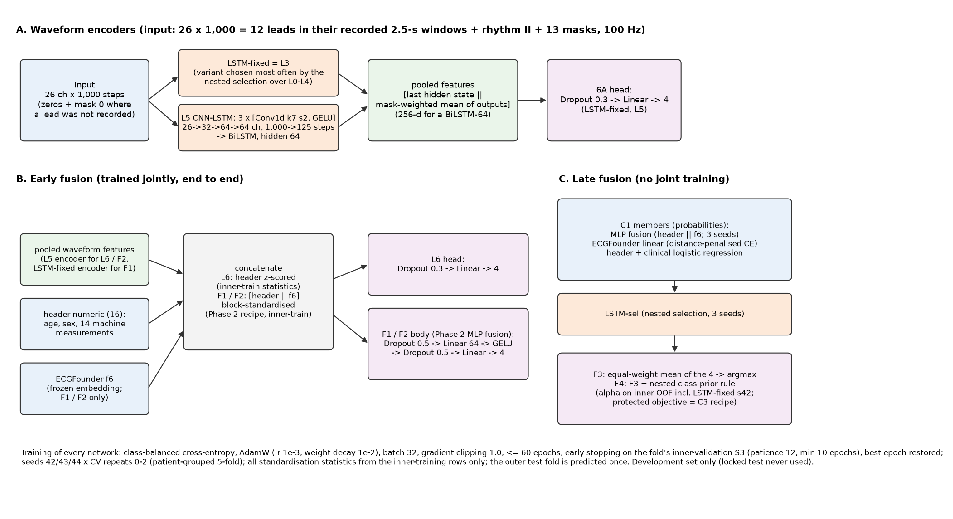
\includegraphics[width=1.00\linewidth,height=0.80\textheight,keepaspectratio]{figures/fig_4_1}
\caption{Phase 6B architectures: waveform encoders (A), early fusion with the header and ECGFounder (B) and late fusion with the vote ensemble (C).}\label{fig:4.1}
\end{figure}

Fine-tuning ECGFounder and adding a second encoder (ECG-FM) did not raise the EF correlation above the frozen embedding ($r\approx0.65$), which confirmed it as the best representation. Phase 6A then built a family of recurrent networks that read the waveform directly (Table~\ref{tab:4.5}): five LSTM variants with 1--2 layers and 64 hidden units, a nested selection among them, and a CNN-LSTM with a three-layer convolutional front-end. The CNN-LSTM had the best screen AUC (0.76) and Mild recall (0.19) of the family with only 117 thousand parameters. Fused with ECGFounder in Phase 6B, the recurrent encoders reached the level of the best ensembles (0.55--0.56, screen AUC 0.83).

\section{Label-quality, cohort and abstention studies}\label{sec:4.4}

Pre-registered studies asked whether cleaner labels, reliable cohorts or abstention could lift performance. On ECGs with clear or verified labels the models score in the 60s and 70s (0.668 on 582 clear-cut ECGs, 0.677 on 620 kept after removing suspect labels, 0.707 on 264 clean, clear-cut ECGs), and selective prediction reaches 0.71 on 22 \% of ECGs. Clinician-style features identified interpretable Mild markers: a spatial QRS--T angle above 100$^{\circ}$ in 52 \% of Mild against 20 \% of Normal ECGs, and poor R-wave progression in 31 \% against 7 \%.

\section{Phase 7 and the image-only ensembles}\label{sec:4.5}

\begin{table}[htbp]
\caption{Label-quality, cohort and abstention studies (development CV).}\label{tab:4.7}
\small
\begin{tabular}{>{\raggedright\arraybackslash\hspace{0pt}}p{\dimexpr 0.404\linewidth-2\tabcolsep\relax}>{\raggedright\arraybackslash\hspace{0pt}}p{\dimexpr 0.303\linewidth-2\tabcolsep\relax}>{\raggedright\arraybackslash\hspace{0pt}}p{\dimexpr 0.291\linewidth-2\tabcolsep\relax}}
\toprule
\textbf{Study} & \textbf{Result} & \textbf{Finding} \\
\midrule
VER: 15 labels corrected to a high-confidence echo & C3 0.565 & label noise costs less than one point \\
HC30: exact-name links within 30 days (395 ECGs) & 0.594; 0.603 with all ECG factors & reliable links give about 0.60 \\
CLEAR: train without 255 border ECGs & 0.668 on the 582 clear-cut ECGs & clear cases are graded well \\
MMCLEAN: remove 217 suspect Mild/Moderate labels & 0.677 on the 620 kept ECGs & accuracy follows label clarity \\
NF / NFS: noise-free training & 0.707 on 264 clean, clear-cut ECGs & strong performance on clean labels \\
MILDFEAT: image-only clinician features & spatial QRS-T angle best single marker & interpretable Mild markers found \\
MILDFIX: Mild-aware, ordinal and EF-based rules & best Mild recall 0.218 at 0.537 & Mild can be traded for accuracy \\
Selective prediction (nested thresholds) & 0.71 on 22 \%, 0.70 on 35 \% answered & confidence is informative \\
\bottomrule
\end{tabular}
\end{table}


\begin{table}[htbp]
\caption{Image-only four-class models (all 837 ECGs, development CV).}\label{tab:4.8}
\small
\begin{tabular}{>{\raggedright\arraybackslash\hspace{0pt}}p{\dimexpr 0.452\linewidth-2\tabcolsep\relax}>{\raggedright\arraybackslash\hspace{0pt}}p{\dimexpr 0.379\linewidth-2\tabcolsep\relax}>{\raggedright\arraybackslash\hspace{0pt}}p{\dimexpr 0.167\linewidth-2\tabcolsep\relax}}
\toprule
\textbf{Model} & \textbf{Accuracy [95 \% CI]} & \textbf{Recall N / Mi / Mo / S} \\
\midrule
HIER: two-stage (Normal / middle / Severe, then Mild vs Moderate) & 0.558 [0.522, 0.594] 0.86 / 0.17 / 0.41 / 0.34 &  \\
HIER-ext (wider tuning grid) & 0.570 [0.527, 0.612] 0.88 / 0.16 / 0.43 / 0.34 &  \\
ENH: synthetic 10-s reconstruction $\rightarrow$ ECGFounder & 0.528 0.76 / 0.18 / 0.44 / 0.41 &  \\
ENH: median-beat shape model & 0.467 0.68 / 0.19 / 0.36 / 0.33 &  \\
ENH: MiniRocket & 0.504 0.74 / 0.22 / 0.38 / 0.33 &  \\
ENH-vote (6 members, tuned class weights) & 0.569 [0.527, 0.610] 0.88 / 0.17 / 0.46 / 0.29 &  \\
\textbf{ULT-stack (10 members + predicted} \textbf{EF)} & \textbf{0.571 [0.542, 0.600]} 0.91 / 0.16 / 0.42 / 0.29 &  \\
ULT2-stack (+ EchoNext-Mini) & 0.569 [0.538, 0.599] 0.90 / 0.15 / 0.44 / 0.28 &  \\
\bottomrule
\end{tabular}
\end{table}


Phase 7 tested new representations and objectives in pilots, measured the learning curve ($+1.4$ accuracy points per doubling of the data) and built header-free cascades. The cascade AGT-img answers only when its EF grade agrees with the image-only classifier and the estimate is far from every class limit: \textbf{0.694 on 56 \%} of ECGs. It was frozen and scored once on the locked test set (\textbf{0.747}). The image-only stacks (HIER, ENH, ULT) then reached 0.570--0.571 without the printed header, above the header-using C3 (0.562).

